\chapter{Subsystem: Environmental Sensing}
%TODO Finish section on environmental sensing

The environmental sensing subsystem includes the air quality sensors and video imaging array. The environmental sensing is an integral function within this vehicle. It is the system that allows operators to gather visual and atmospheric information, an essential component for assessing scene safety. In addition the air quality sensors must display accurate information because they determine what gear is required to enter the area. The video imaging array is critical as it allows the operator to successfully see where the vehicle is within the environment, thus making it easy for the operator to drive through and visually inspect the environment. 

\section{Air Quality Assessment}

The air quality sensing subsystem consists of three redundant packages distributed across the vehicle. Using three independent but redundant packages will improve accuracy of results since operators then have multiple values to compare against if there is a spike. It will also allow a safety buffer if one or more sensors were to fail. Within each package there will be five or more sensors. The base list of gas sensors includes: Carbon Monoxide, Carbon Dioxide, Liquid Petroleum Gas, Methane, and air particulate. Additionally, there will be atemperature sensor that can read temperatures in excess of 200\degree F and a humidity sensor. 

\subsection{Payload Requirements}
%High level requirements that led to design

\subsection{Component Selection}
%Why we chose the various sensors

\subsection{PCB Design}
%Mounted everything on custom PCB
%Problems that occurred after manufacturing
%include PCB layout and picture

\subsection{Manufacturing and Assembly}
%Include pictures of PCB in assembly

\subsection{Calibration Procedure}

\subsection{Data Processing}
%Potential subsection if turns out to be long
%Flowdown of arduino code
%Communication to ROS

\section{Cameras}

The camera system is a four camera array that provides a front facing view for the operator as well as a roughly 260\degree  view for observation of the surroundings. The initial design included four IP cameras, all of which run as a unique node within the ROS network. ROS handles IP cameras over RTSP, the Real Time Streaming Protocol. This introduced an unacceptable amount of latency, about 4 seconds, to the camera stream. The final design includes four Logitech c615 usb cameras that are connected to a Raspberry Pi 2 Model B. A photo of the selected model of Logitech camera is included in Figure \ref{fig:logitechcam}. The dedicated Raspberry Pi runs an image of Ubuntu with ROS. The usb camera images are captured through ROS and sent through an OpenCV "person detection" application that recognizes bodies within the camera stream and outlines them in a green box so that they are visible to the operator. For an example of this capability, see Figure \ref{fig:peopledetect}. 

\begin{figure}[H]
	\centering
	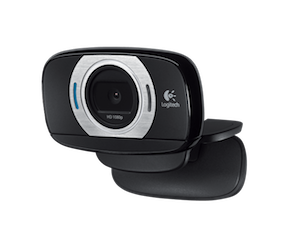
\includegraphics[scale=1]{c615.png}
	\caption{Logitech c615 camera}
	\label{fig:logitechcam}
\end{figure}
\begin{figure}[H]
	\centering
	\includegraphics[scale=1]{pepoledetection.jpg}
	\caption{Example of OpenCV People Detection Application}
	\label{fig:peopledetect}
	\end{figure}

\section{Sensor and Camera Layout}
%TODO Include picture of layout

The location of the air quality sensors and cameras was a design decision. For the cameras, the field of view, mounting costs, implementation time and robustness, among other factors, were considered when deciding on a final design. Additionally, for the environmental sensors, the cost, implementation time, robustness and proximity to the vehicle's exhaust systems were considered when deciding on a sensor configuration. Appendix \ref{App:tradeoff} features a complete tradeoff analysis for the sensor configurations. A final configuration was chosen where the cameras are mounted on all 4 corners of the roll cage, allowing for a 360 degree view of the surroundings while also allowing the operator to see over obstacles. The redundant sensor packages will be located on either side of the roll cage and on the front of the vehicle. 

\section{Summary}